\section{Hardware Introduction}
\hyperdef{hw}{introduction}{[Marker:hw.introduction]}\\
\subsection{Demonstrator}
\subsubsection{Front End Electronics board FEE}
\begin{figure}[htb]
\centering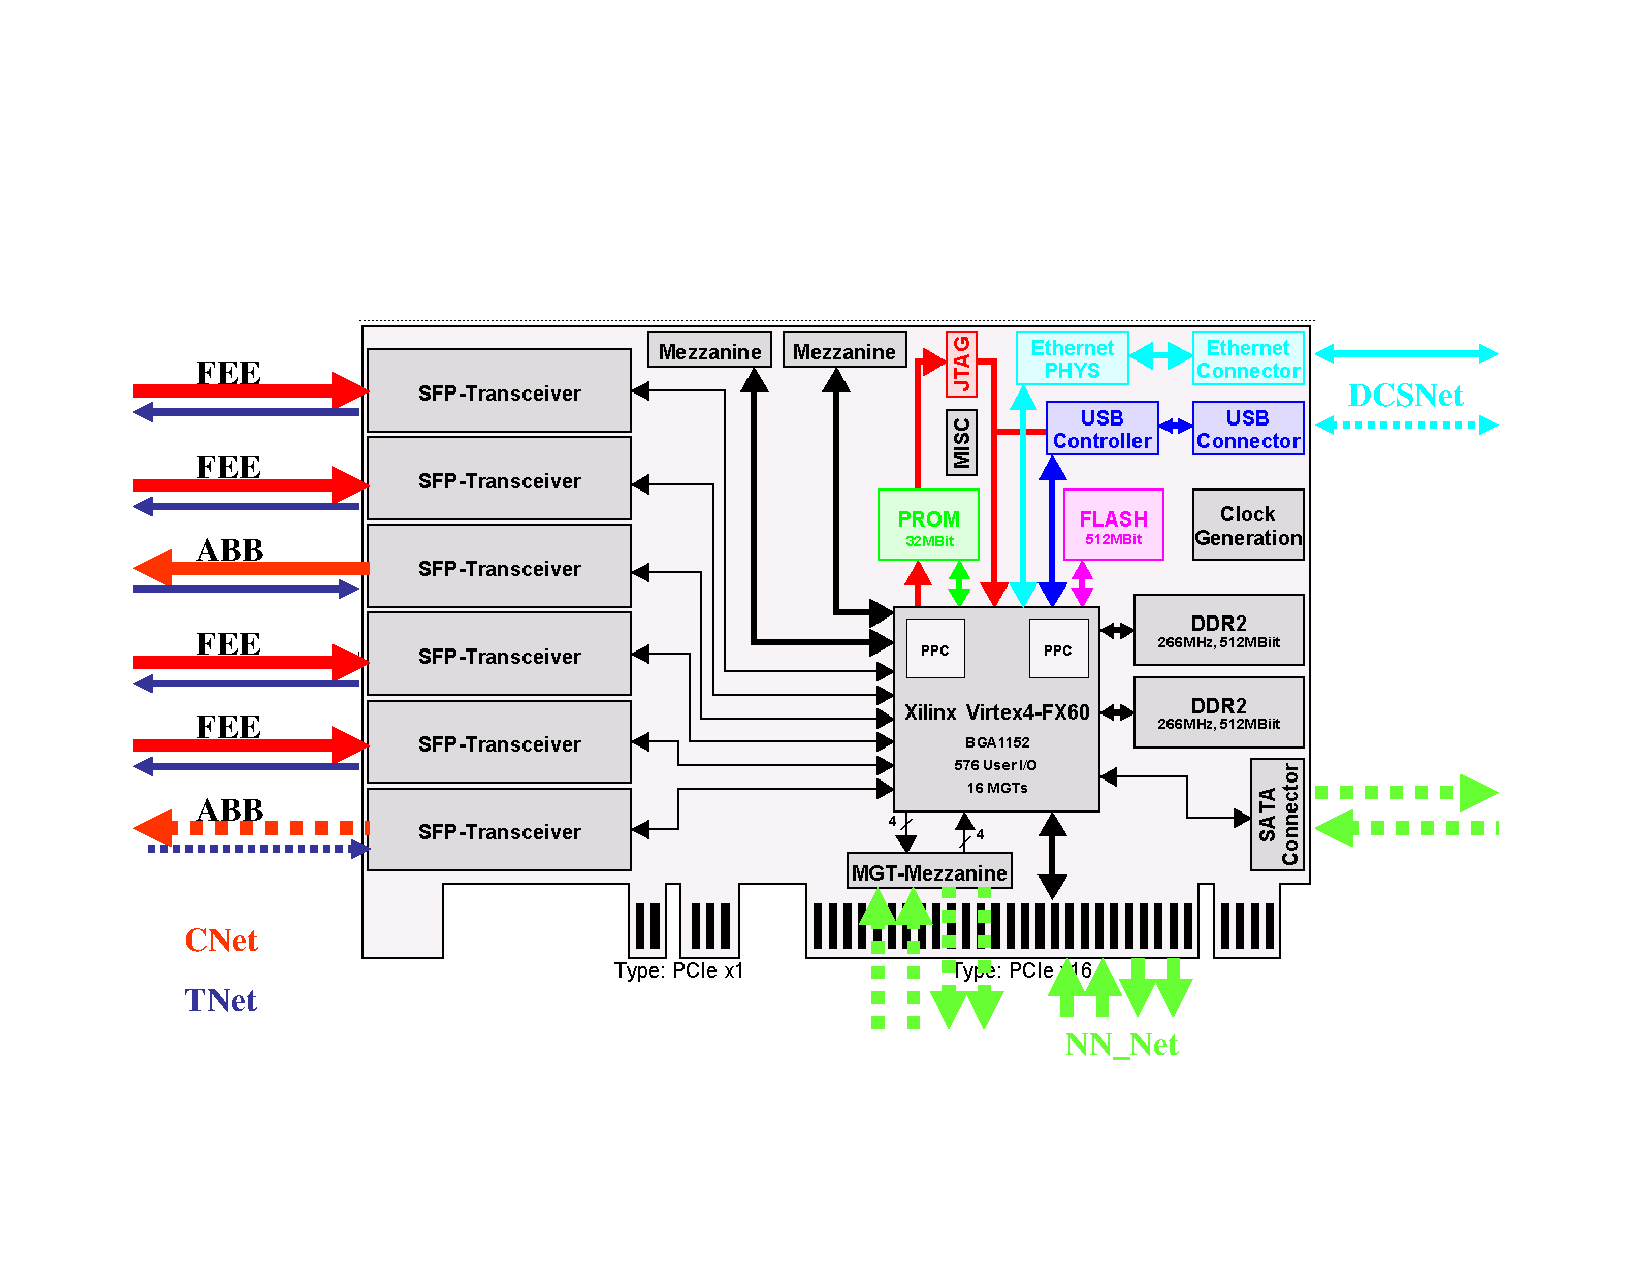
\includegraphics[width=.8\textwidth]
{demof-dcb} \caption{Scetch of FPGA board (Br\" uning)}
\label{fig:dcb}
\end{figure}
General purpose chamber-mountable board with ADCs (4*4 channels,
65 MHz sampling, 10-12 bit), FPGA (Virtex-4, PPC, Ethernet MAC,
MGT plus SDRAM, CPLD, NVRAM), plugable to preamp/chapers. A
version utilizing pipeline TDCs (ns resolution) possible. Two
clock domains: receive clock of 312.5 MHz (timing and trigger) and
sampling clock with 62.5 MHz (measurement). Four pair of LVDS
bi-directional links (625 Mbps).
\subsubsection{Data Combiner board DCB}
Four bi-directional LVDS links to FEB, Ethernet, MGT with SFP
optical link to ABB, same FPGA. A test layout of such board is shown in Fig.~\ref{fig:dcb}.
A possible connection to the between FEE and DCB boards is shown if Fig.~\ref{fig:fee-dcb}
\subsubsection{Active Buffer board ABB}
PCIe board, 4 - 8 MGT/SFP optical links to DCBs, same FPGA.
\subsubsection{Timing board}
Similar to DCB, gets optional trigger inputs, generates clock and distributes through
optical splitters to DCBs.
\subsubsection{Event builder}
Standard PC with GE, InifiniBand switch.
\begin{figure}[htb]
\centering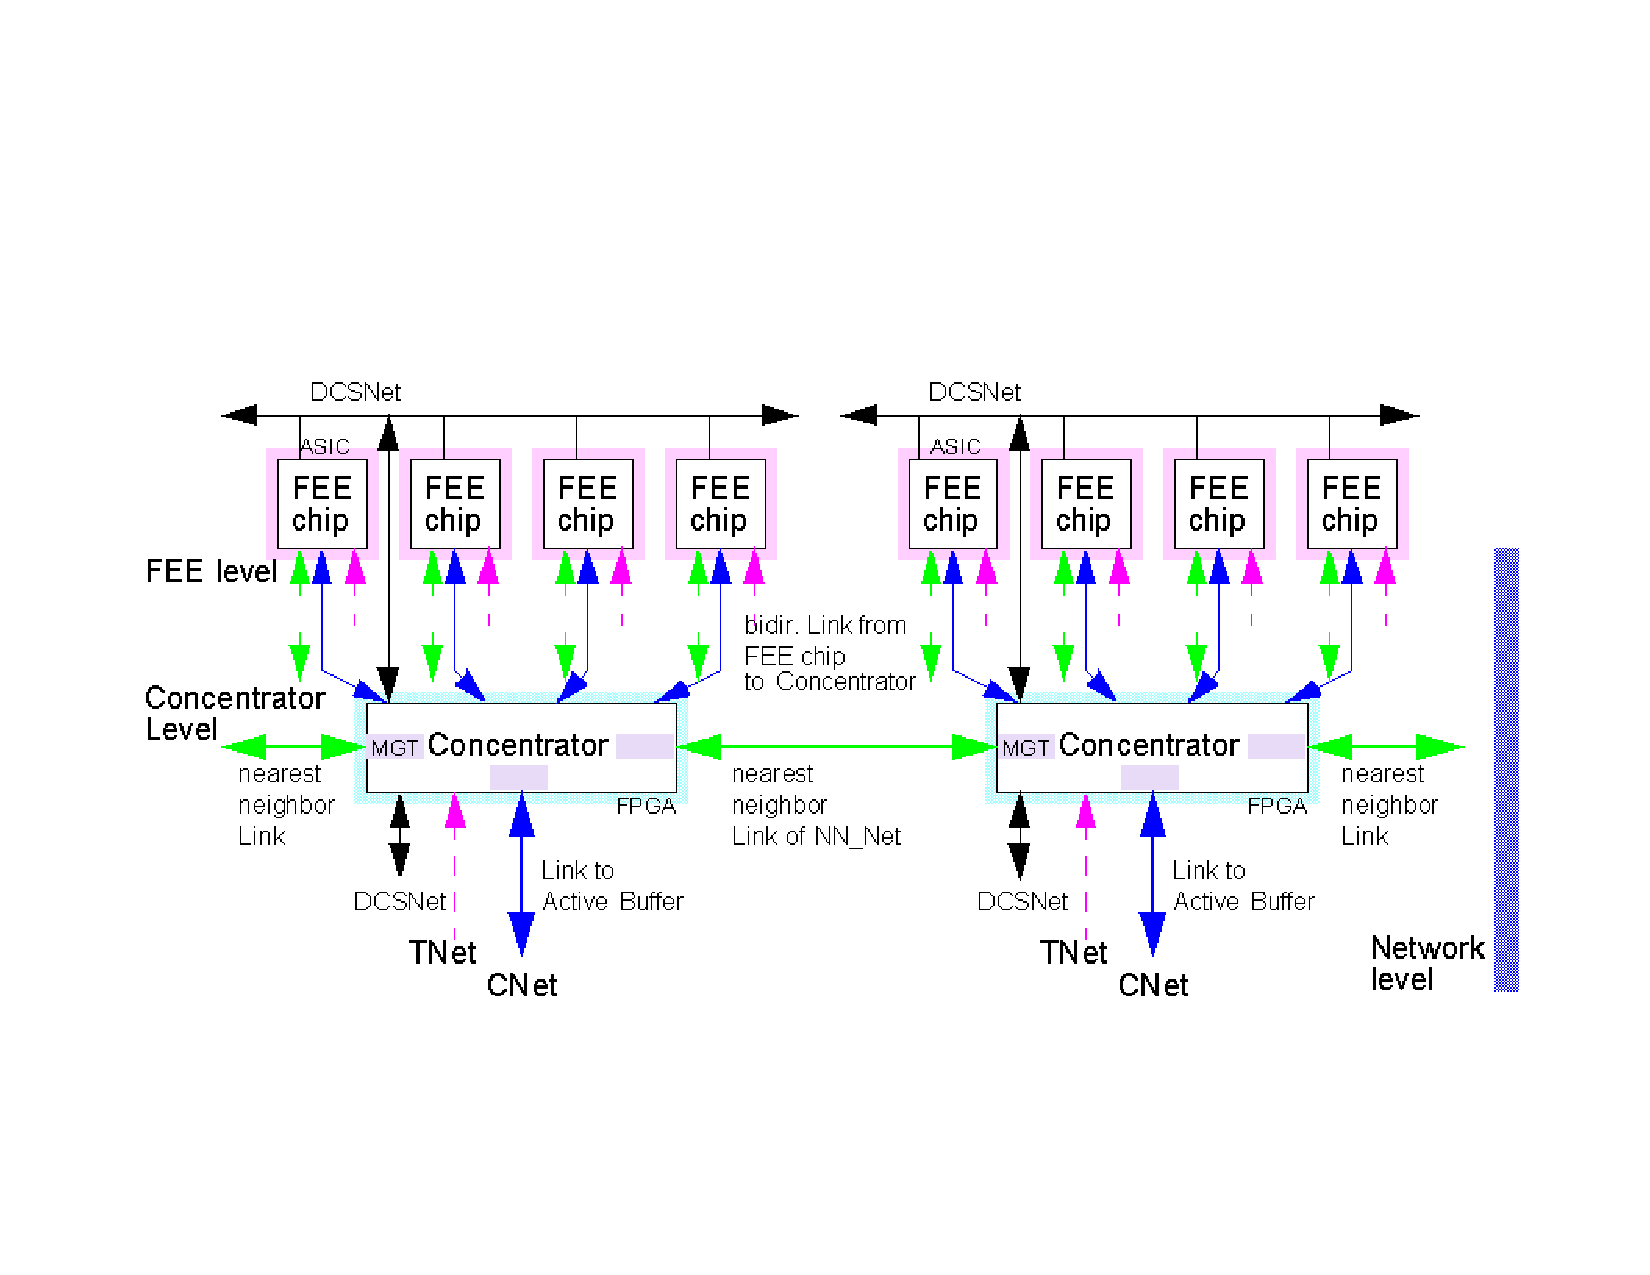
\includegraphics[width=.8\textwidth]
{demof-fee-dcb}
\caption{FEE and DCB connections}
\label{fig:fee-dcb}
\end{figure}
